\documentclass{article}
\usepackage{graphicx} % Required for inserting images
\usepackage{tikz}
\usepackage[landscape]{geometry}
\usepackage{float}
\usepackage{listings}
\usepackage{caption}
\usepackage{subcaption}

%arrange page numbers
\usepackage{fancyhdr}
\pagestyle{fancy}
\fancyhf{}
\renewcommand{\headrulewidth}{0pt}
\fancyhead[R]{\thepage}

%setup Tikz to draw the graphs
\usetikzlibrary{external}
\tikzexternalize 
%load options
\usetikzlibrary{positioning, calc, shapes.geometric, shapes.multipart,
        shapes, arrows.meta, arrows, decorations.markings, external, trees}

%Create custom arrow style:
\tikzstyle{Arrow} = [
thick,
decoration={
markings,
mark=at position 0.9999 with {
\arrow[thick]{latex}}},
shorten >= 3pt, preaction = {decorate}]




\title{Tikz DAGs}
\author{tpfeeney }
\date{June 2023}

\begin{document}


\section{Figure 1}

\begin{figure}[H]
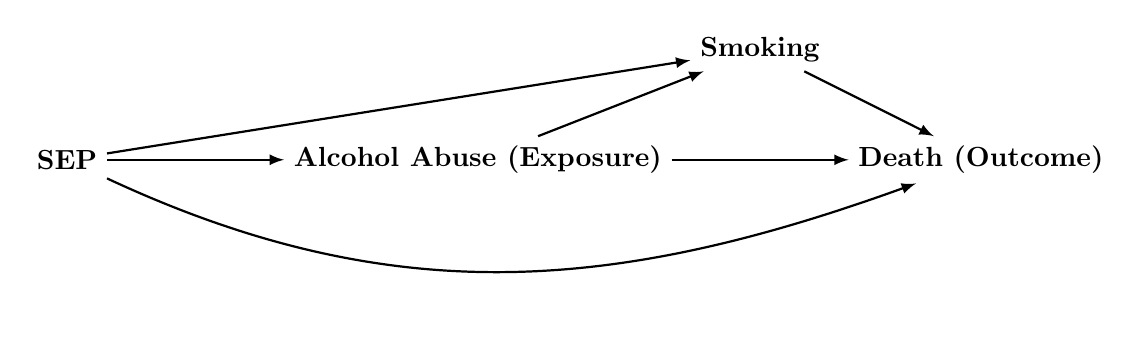
\begin{tikzpicture}
    \node (1) {};
    \node [right =of 1] (2)  {\textbf{Alcohol Abuse (Exposure)}};
    \node [right =of 2] (3) {};
    \node [right =of 3] (4) {\textbf{Death (Outcome)}};
    \node [left =of 1] (5) {\textbf{SEP}};
    \node [above =of 3] (6) {\textbf{Smoking}};

    \draw[Arrow] (2.east)--(4.west);
    \draw[Arrow] (2) to (6);
    \draw[Arrow] (6) to (4);
    \draw[Arrow] (5) to [out=-25, in=-160] (4);
    \draw[Arrow] (5) to (6);
    \draw[Arrow] (5.east)--(2.west);
\end{tikzpicture}
\caption{An example of a DAG with exposure to alcohol abuse, Outcome death, confounder socioeconomic position, and mediator smoking.}
\end{figure}

\section{Figure 2}

\begin{figure}[H]
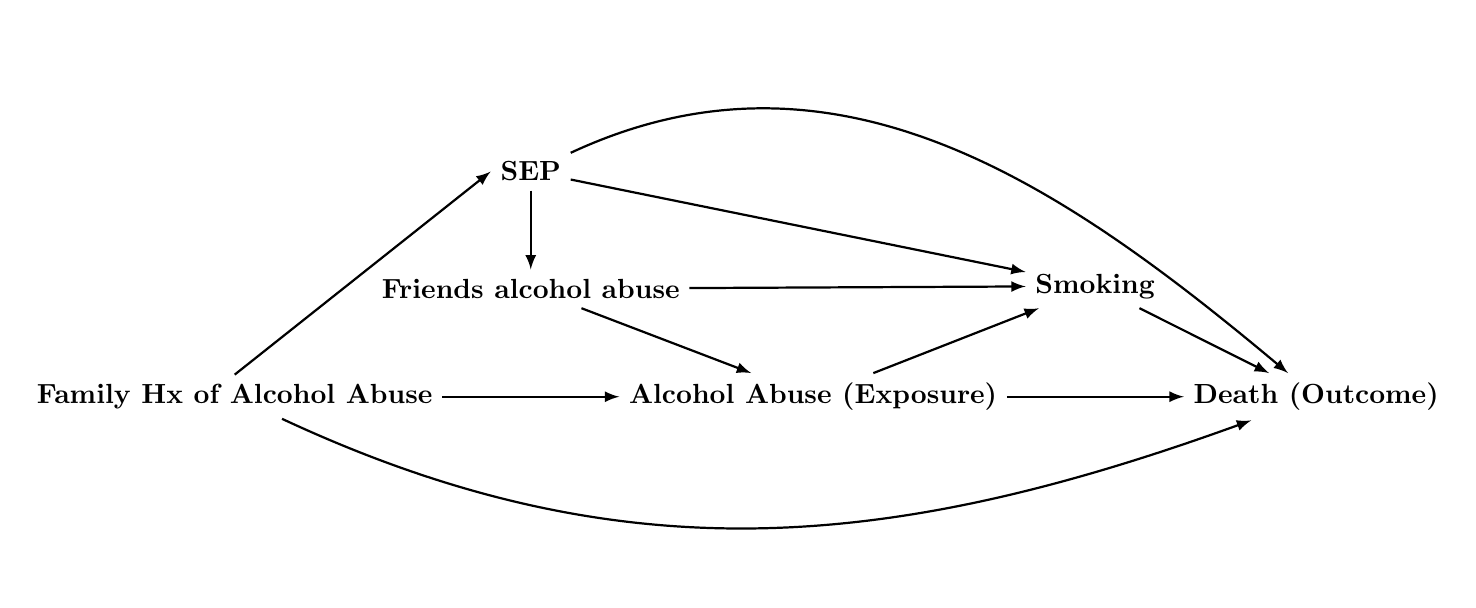
\begin{tikzpicture}
    \node (1) {\textbf{Family Hx of Alcohol Abuse}};
    \node [above =of 1] (11) {};
    \node [above =of 11] (12) {};
    \node [above =of 12] (13) {};
    \node [right =of 1] (2) {};
    \node [above =of 2] (10) {\textbf{Friends alcohol abuse}};
    \node [above =of 10] (8) {\textbf{SEP}};
    \node [right =of 2] (3) {\textbf{Alcohol Abuse (Exposure)}};
    \node [above =of 3] (9) {};
    \node [right =of 8] (7) {};
    \node [right =of 3] (4) {};
    \node [above =of 4] (6) {\textbf{Smoking}};
    \node [right =of 4] (5) {\textbf{Death (Outcome)}};
    \draw[Arrow] (3.east)--(5.west);
    \draw[Arrow] (3) to (6);
        \draw[Arrow] (6) to (5);
    \draw[Arrow] (1) to (3);
        \draw[Arrow, thick] (1.north)--(8.west);
        \draw[Arrow] (1) to [out=-25, in=-160] (5);
    \draw[Arrow] (8) to (6);
    \draw[Arrow] (8) to [out=25, in=140] (5);
    \draw[Arrow] (10) to (6);
    \draw[Arrow] (10) to (3);
    \draw[Arrow] (8) to (10);
\end{tikzpicture}
\caption{Family history of alcohol abuse, socioeconomic position, and friends’ alcohol abuse are confounders; smoking is a mediator, alcohol abuse is the exposure of interest, and mortality is the outcome of interest.}
\label{fig: Figure 2}
\end{figure}

\section{Figure 3}

\begin{figure}[H]
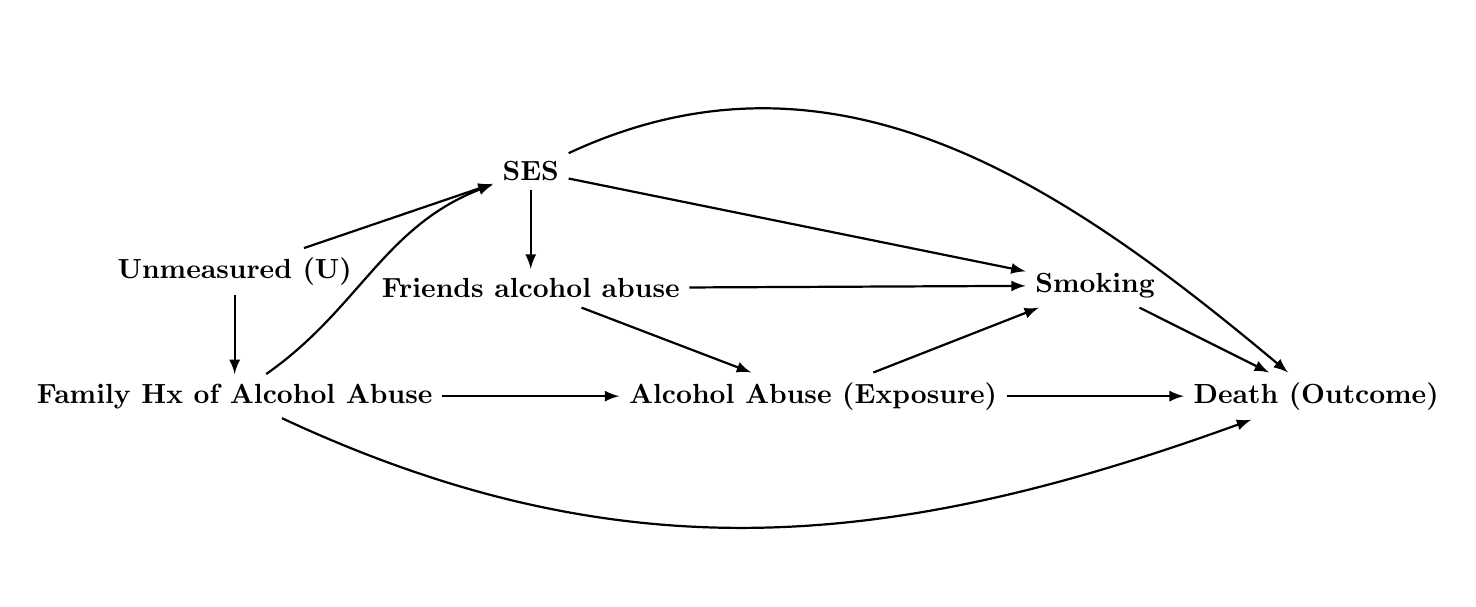
\begin{tikzpicture}
    \node (1) {\textbf{Family Hx of Alcohol Abuse}};
    \node [above =of 1] (11) {};
    \node [above =of 11] (12) {};
    \node [above =of 12] (13) {};
    \node [right =of 1] (2) {};
    \node [above =of 2] (10) {\textbf{Friends alcohol abuse}};
    \node [above =of 10] (8) {\textbf{SES}};
    \node [right =of 2] (3) {\textbf{Alcohol Abuse (Exposure)}};
    \node [above =of 3] (9) {};
    \node [right =of 8] (7) {};
    \node [right =of 3] (4) {};
    \node [above =of 4] (6) {\textbf{Smoking}};
    \node [right =of 4] (5) {\textbf{Death (Outcome)}};
    \node [above =of 1] (14) {\textbf{Unmeasured (U)}};
    \draw[Arrow] (3.east)--(5.west);
    \draw[Arrow] (3) to (6);
        \draw[Arrow] (6) to (5);
    \draw[Arrow] (1) to (3);
        \draw[Arrow, thick] (1) to [out=35, in=-160] (8);
        \draw[Arrow] (1) to [out=-25, in=-160] (5);
    \draw[Arrow] (8) to (6);
    \draw[Arrow] (8) to [out=25, in=140] (5);
    \draw[Arrow] (10) to (6);
    \draw[Arrow] (10) to (3);
    \draw[Arrow] (8) to (10);
    \draw[Arrow] (14) to (1);
    \draw[Arrow] (14) to (8);
\end{tikzpicture}
\caption{The DAG from Figure 2 with an unmeasured confounder. In this case, U is either unknown or unmeasured but is a common cause of a family history of alcohol abuse and smoking.}
\end{figure}



\section{Figure 4}
\begin{figure}[H]
\subsection{Figure 4a}
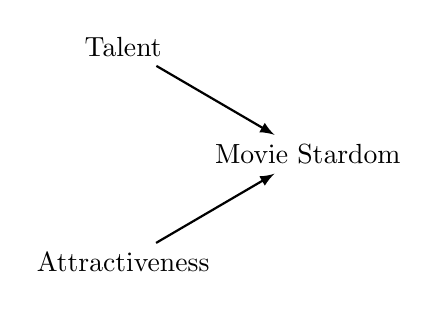
\begin{tikzpicture}
    \node (1) {Attractiveness};
    \node  [right =of 1] (2) {};
    \node [right =of 2] (3)  {};
    \node [above =of 2] (4) {Movie Stardom};
    \node [above =of 1] (6) {};
    \node [above =of 6] (7) {Talent};

    \draw[Arrow] (7) to (4);
    \draw[Arrow] (1) to (4);
\end{tikzpicture}

\subsection{Figure 4b}
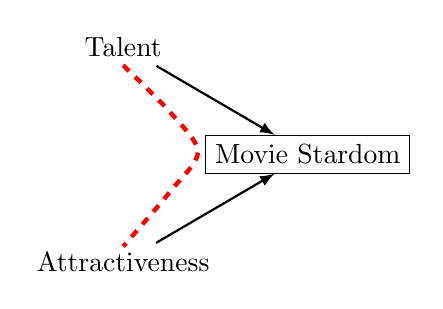
\begin{tikzpicture}
    \node (1) {Attractiveness};
    \node  [right =of 1] (2) {};
    \node [right =of 2] (3)  {};
    \node [rectangle, draw, above =of 2] (4) {Movie Stardom};
    \node [above =of 1] (6) {};
    \node [above =of 6] (7) {Talent};
    \draw[Arrow] (7) to (4);
    \draw[Arrow] (1) to (4);
    \draw [smooth, ultra thick, dashed, red] plot coordinates{(0,2.5)(0.6,1.9)(0.95,1.40)(0.6,0.9)(0,0.2)};
\end{tikzpicture}
\caption{A) Movie stardom is a collider without adjustment, there is no relationship between  a attractiveness and talent B) After adjustment for the collider, there is an induced relationship between talent and attractiveness (red dashed line) through movie stardom, which is not truly causal.}
\end{figure}

\section{Figure 5}

\begin{figure}[H]
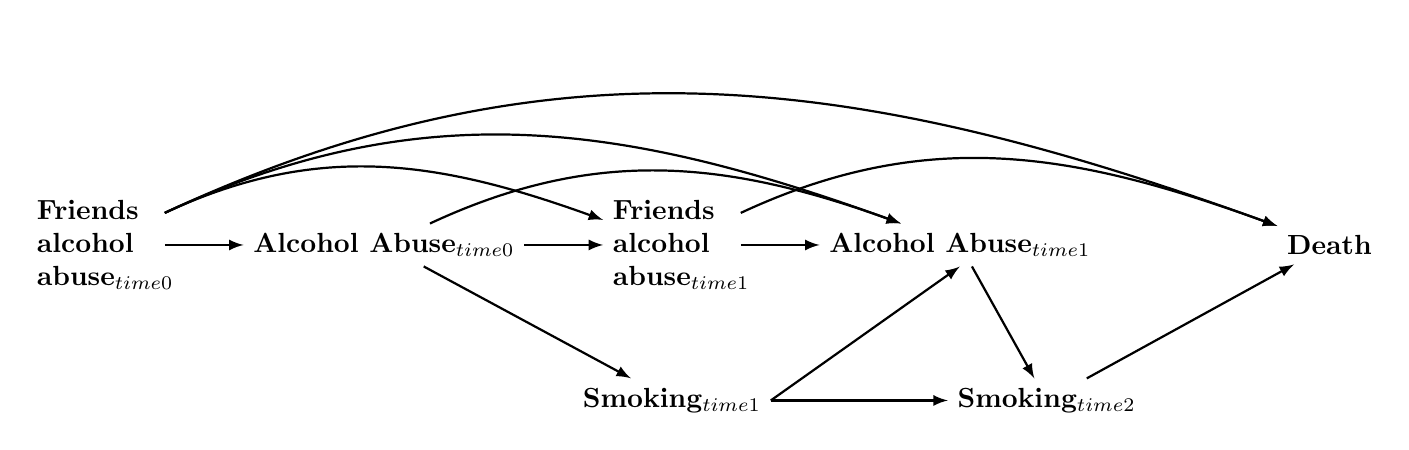
\begin{tikzpicture}
    \node [text width=1.5cm](1) {\textbf{Friends alcohol abuse$_{time 0}$}};
    \node [right =of 1] (2) {\textbf{Alcohol Abuse$_{time 0}$}};
    \node [right =of 2,text width=1.5cm] (3) {\textbf{Friends alcohol abuse$_{time 1}$}};
    \node [right =of 3] (4) {\textbf{Alcohol Abuse$_{time 1}$}};
    \node [right =of 4] (5) {};
    \node [right =of 5] (8) {\textbf{Death}};
    \node [below =of 3] (6) {\textbf{Smoking$_{time 1}$}};
    \node [right =of 6] (9) {};
    \node [right =of 9] (7) {\textbf{Smoking$_{time 2}$}};
    \draw[Arrow, thick] (1.east) -- (2.west);
    \draw[Arrow, thick] (1) to [out=25, in=160] (3);
    \draw[Arrow, thick] (1) to [out=25, in=160] (4);
    \draw[Arrow, thick] (1) to [out=25, in=160] (8);
    \draw[Arrow, thick] (2.east) -- (3.west);
    \draw[Arrow, thick] (2) to [out=25, in=160] (4);
    \draw[Arrow, thick] (3.east) -- (4.west);
    \draw[Arrow, thick] (3) to [out=25, in=160] (8);
    \draw[Arrow, thick] (2) to (6);
    \draw[Arrow, thick] (6.east) -- (4.south);
    \draw[Arrow, thick] (6.east) -- (7);
    \draw[Arrow, thick] (4) to (7);
    \draw[Arrow, thick] (7) to (8);
\end{tikzpicture}
\caption{Time Variant DAG with the exposure to alcohol abuse was measured at baseline, and a later follow-up (Alcohol abuse$_{time 1}$, and smoking and friends who abuse alcohol were also measured at baseline and follow-up. The outcome is unchanged and is 5-year mortality (Death).}
\end{figure}


\section{Figure 6}

\begin{figure}[H]

\subsection*{A}
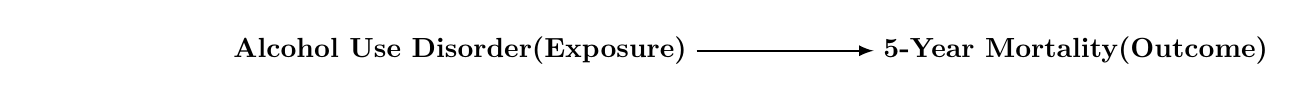
\begin{tikzpicture}
    \node (1) {};
    \node [right =of 1] (2) {};
    \node [right =of 2] (3) {\textbf{Alcohol Use Disorder(Exposure)}};
    \node [right =of 3] (4) {};
    \node [right =of 4] (5) {\textbf{5-Year Mortality(Outcome)}};
    \draw[Arrow] (3.east)--(5.west);
\end{tikzpicture}

\subsection*{B}
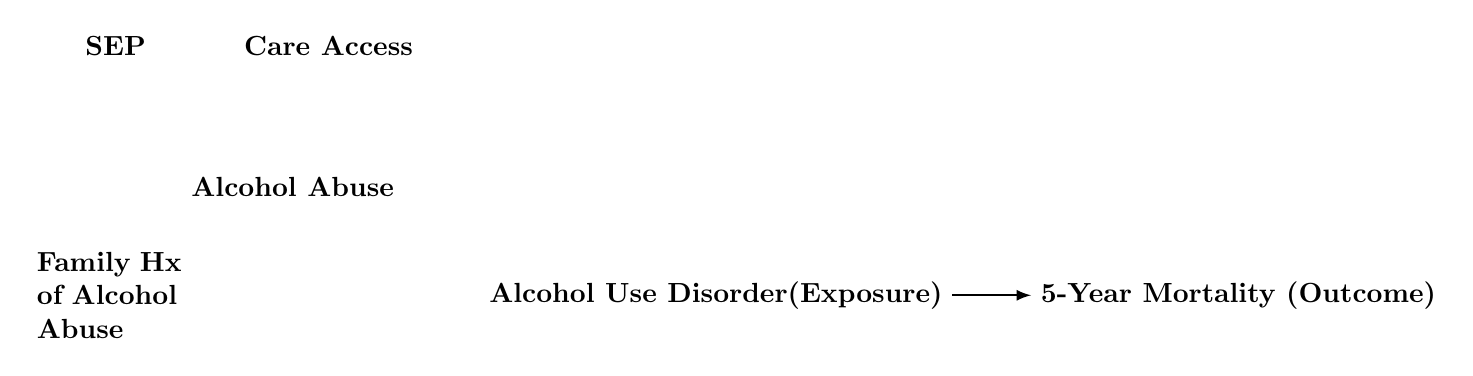
\begin{tikzpicture}
    \node (1) [text width=2cm] {\textbf{Family Hx of Alcohol Abuse}};
    \node [right =of 1] (2) {};
    \node [right =of 2] (3) {};
    \node [right =of 3] (4) {\textbf{Alcohol Use Disorder(Exposure)}};
    \node [right =of 4] (6) {\textbf{5-Year Mortality (Outcome)}};
    \node [above =of 1] (13) {};
    \node [above =of 2] (9) {\textbf{Alcohol Abuse}};
    \node [above =of 13] (7) {\textbf{SEP}};
    \node [right =of 7] (8) {\textbf{Care Access}};
    \draw[Arrow] (4.east)--(6.west);
\end{tikzpicture}
\end{figure}
%need to split these up to smaller figures
\setcounter{figure}{5} %this resets counter so both smaller figures are Figure 6.

\begin{figure}[H]
\subsection*{C}
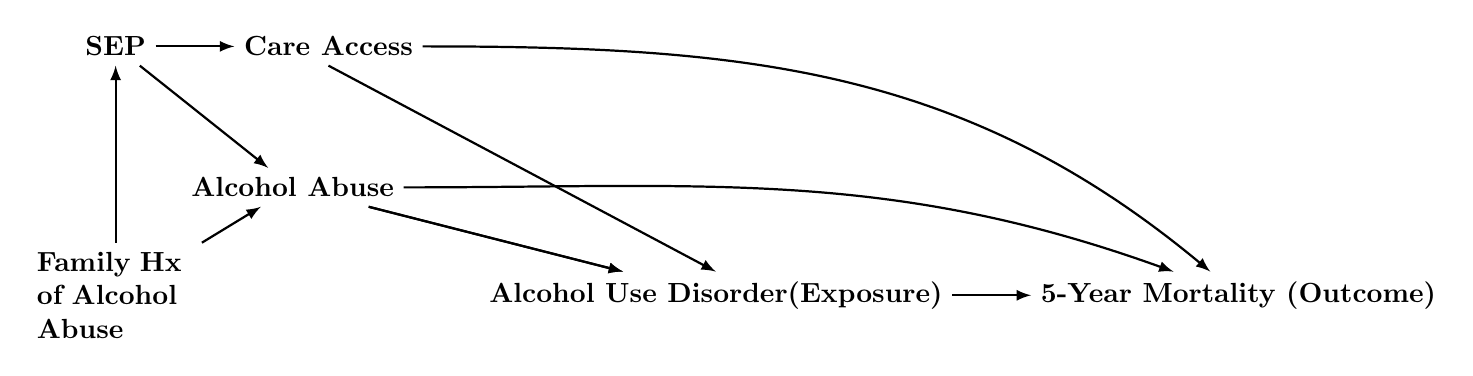
\begin{tikzpicture}
    \node (1) [text width=2cm] {\textbf{Family Hx of Alcohol Abuse}};
    \node [right =of 1] (2) {};
    \node [right =of 2] (3) {};
    \node [right =of 3] (4) {\textbf{Alcohol Use Disorder(Exposure)}};
    \node [right =of 4] (6) {\textbf{5-Year Mortality (Outcome)}};
    \node [above =of 1] (13) {};
    \node [above =of 2] (9) {\textbf{Alcohol Abuse}};
    \node [above =of 13] (7) {\textbf{SEP}};
    \node [right =of 7] (8) {\textbf{Care Access}};
    \draw[Arrow] (4.east)--(6.west);
    \draw[Arrow] (1.north) to (7.south);
    \draw[Arrow] (7.east) to (8.west);
    \draw[Arrow] (7) to  (9);
    \draw[Arrow] (9) to  (4);
    \draw[Arrow] (8) to [out=0, in=140] (6);
    \draw[Arrow] (8.south) to  (4.north);
    \draw[Arrow] (9) to  (4);
    \draw[Arrow] (9) to [out=0, in=160]  (6);
    \draw[Arrow] (1) to (9);
    
\end{tikzpicture}

\subsection*{D}
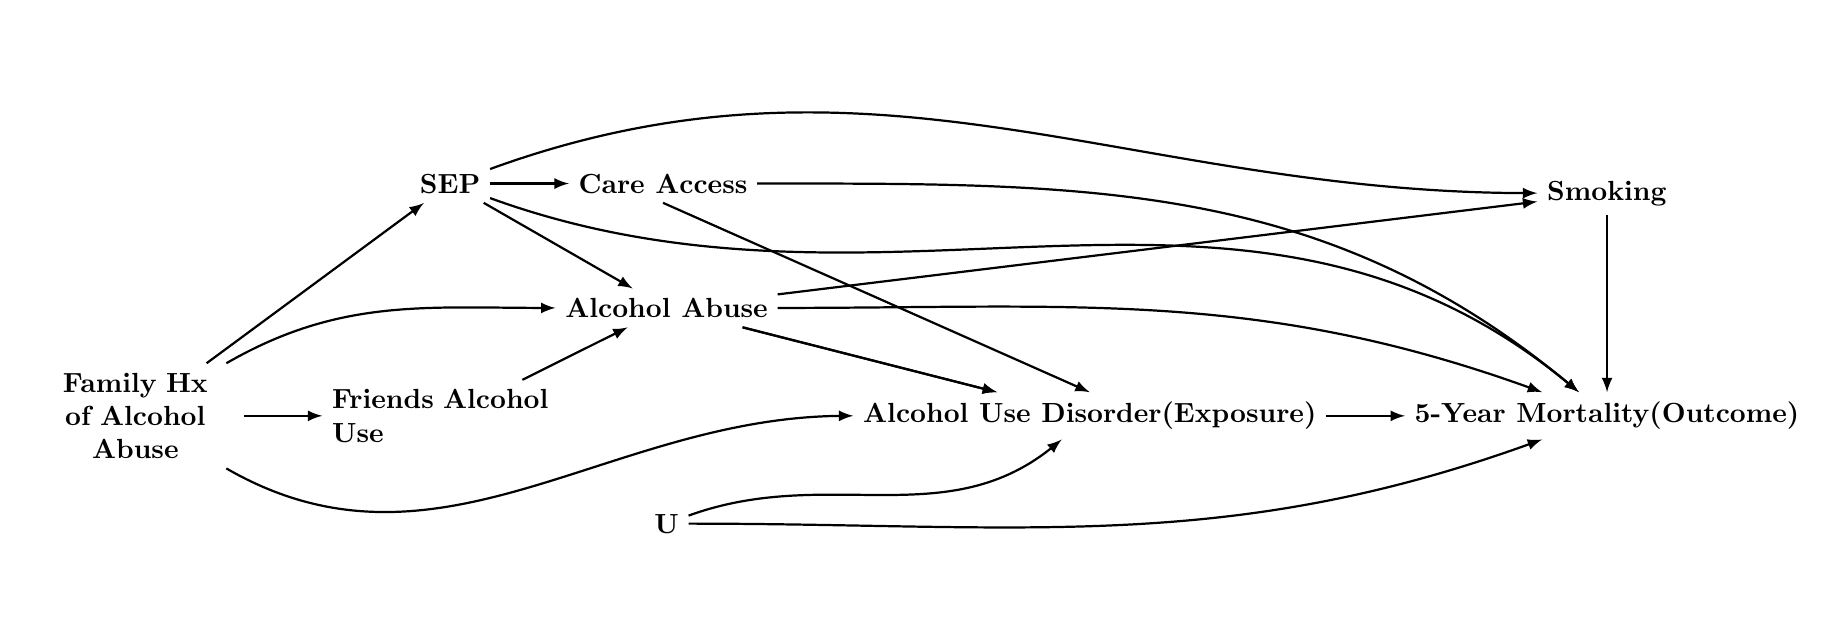
\begin{tikzpicture}
    \node (1) [text width=3cm] {\textbf{Friends Alcohol Use}};
    \node [right =of 1] (2) {};
    \node [right =of 2] (3) {};
    \node [right =of 3] (4) {\textbf{Alcohol Use Disorder(Exposure)}};
    \node [right =of 4] (6) {\textbf{5-Year Mortality(Outcome)}};
    \node [above =of 1] (13) {};
    \node [above =of 2] (9) {\textbf{Alcohol Abuse}};
    \node [above =of 13] (7) {\textbf{SEP}};
    \node [right =of 7] (8) {\textbf{Care Access}};
    \node [above =of 6] (15) {};
    \node [above =of 15] (16) {\textbf{Smoking}};
    \node [below =of 2] (17) {\textbf{U}};
    \node [left =of 1, text width=2.5cm,align=center] (18) {\textbf{Family Hx of Alcohol Abuse}};
    \draw[Arrow] (4.east)--(6.west);
    \draw[Arrow] (18.east) to (1.west);
    \draw[Arrow] (7.east) to (8.west);
    \draw[Arrow] (7) to  (9);
    \draw[Arrow] (9) to  (4);
    \draw[Arrow] (8) to [out=0, in=140] (6);
    \draw[Arrow] (8.south) to  (4.north);
    \draw[Arrow] (9) to  (4);
    \draw[Arrow] (9) to [out=0, in=160]  (6);
    \draw[Arrow] (1) to (9);
    \draw[Arrow] (7) to [out=20, in=180] (16);
    \draw[Arrow] (9) to (16);
    \draw[Arrow] (16) to (6);
    \draw[Arrow] (17) to [out=20, in=-140] (4);
    \draw[Arrow] (17) to [out=0, in=-160](6);
    \draw [Arrow] (7) to [out=-20, in=140] (6);
    \draw [Arrow] (18) to (7);
    \draw [Arrow] (18) to [out=30, in=180] (9);
    \draw [Arrow] (18) to [out=-30, in=-180] (4);
\end{tikzpicture}


\caption{Process of constructing a DAG. A) The process starts with defining the exposure and outcome of interest. B) Initial DAGs can be constructed using expert knowledge and previous studies to inform variables that are related to both the exposure and outcome, but also other variables. C) Refinement and consensus help complete the DAG including all relationships between variables and the exposure and outcome. Exp=exposure, SEP=Socioeconomic Position, Hx=history, U=unmeasured and possibly unknown.}
\end{figure}

%%%Figure 7
\section*{Figure 7}
\subsection*{A}
\begin{figure}[H]
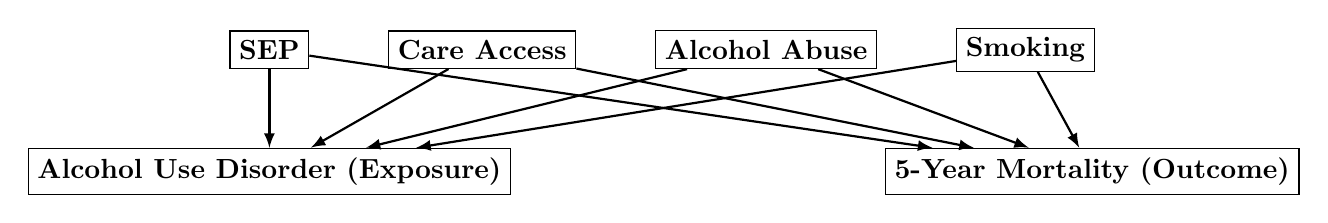
\begin{tikzpicture}
    \node [rectangle, draw](1) {\textbf{Alcohol Use Disorder (Exposure)}};
    \node [right =of 1] (2) {};
    \node [right =of 2] (3) {};
    \node [right =of 3] (4) {};
    \node [right =of 4, rectangle, draw] (5) {\textbf{5-Year Mortality (Outcome)}};
    \node [above =of 1, rectangle, draw] (6) {\textbf{SEP}};
    \node [right =of 6, rectangle, draw] (7) {\textbf{Care Access}};
    \node [right =of 7, rectangle, draw] (8) {\textbf{Alcohol Abuse}};
    \node [right =of 8, rectangle, draw] (9) {\textbf{Smoking}};
    \draw [Arrow] (6) to (1); \draw [Arrow] (6) to (5);
    \draw [Arrow] (7) to (1); \draw [Arrow] (7) to (5);
    \draw [Arrow] (8) to (1); \draw [Arrow] (8) to (5);
    \draw [Arrow] (9) to (1); \draw [Arrow] (9) to (5);
\end{tikzpicture}

\subsection*{B}
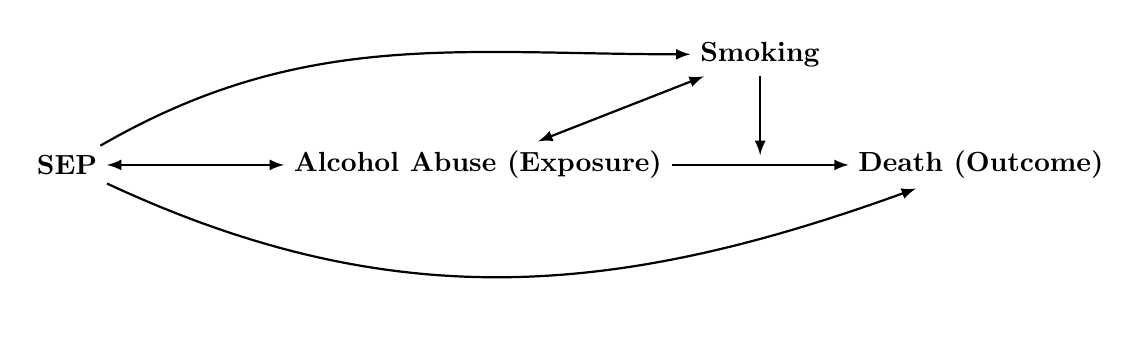
\begin{tikzpicture}
    \node (1) {};
    \node [right =of 1] (2)  {\textbf{Alcohol Abuse (Exposure)}};
    \node [right =of 2] (3) {};
    \node [right =of 3] (4) {\textbf{Death (Outcome)}};
    \node [left =of 1] (5) {\textbf{SEP}};
    \node [above =of 3] (6) {\textbf{Smoking}};

    \draw[Arrow] (2.east)--(4.west);
    \draw[>=latex, thick, <->] (2)--(6);
    \draw[Arrow] (6) to (3);
    \draw[Arrow] (5) to [out=-25, in=-160] (4);
    \draw[Arrow] (5) to [out=30, in=180] (6);
    \draw[>=latex, thick, <->] (5.east)--(2.west);
\end{tikzpicture}
\end{figure}

\end{document}
